% future_developements.tex

We have stepped through, in detail, the low-mass \ac{CBC} pipeline, and we have
described how this was used to obtain search results from \acp{CBC}. We now
conclude by briefly presenting some future developements for the pipeline.

\section{Gating}

In chapter \ref{ch:s6_results} we saw the effects a loud transient --- the
spike glitch --- had on the matched filter. We dealt with the spike glitch by
adding a category 3 veto around the time of the glitch. Due to the ringing of
the filter we had to add a $\pm 8\,$s padding to the glitch. However, as can be
seen in figure \ref{fig:spike_glitch-cbc_response}, triggers can be last for
several tens of seconds after the glitch; this duration increases with the size
of the glitch.

Another possibility is to remove the glitch \emph{prior} to match filtering. We
can do this by applying a Tukey window to the data stream to ramp the output
down to $0$ at the time of the glitch. We call this ``gating." Figure
\ref{fig:gating-time_series} shows a time series in which a spike-glitch
occurred with a gate applied.  In \ref{fig:gating-time_series-gated} the window
that is applied can be seen. We must ramp the data down (in this case, by using
the first half cycle of a cosine) so as not to introduce ringing at the point
the window turns on, and we must do the same after the glitch to ramp the data
back up. In this manner we can cleanly remove the glitch from the data: compare
the Omega scans in Figure \ref{fig:gating-omega_scans} with the glitch in the
data to the scan with the glitch gated out.

Zeroing out the data around the glitch does mean that we will slightly
underestimate the \ac{PSD}. However, if the gated data is only a few seconds
out of an entire analysis block, the effect should be small. It may also be
possible to correct for the zeroed out data by taking the average power across
the segment, then add a correction factor. Even if we add a correction factor
to the \ac{PSD}, we should probably limit the amount of time that is gated in
an analysis block. The upper limit on how much time can gated in a block
requires more study.

Knowing what to gate also needs study. In the case of the spike glitch, we
could not find the cause, as we could not correlate it with any auxiliary
environmental or instrumental channels. We got around this difficulty by
applying the \ac{SNR} $> 250$ flag at CAT3, which allowed us to check the
results at CAT2 to ensure we did not accidentally veto a loud \ac{GW} trigger.
Since gating involves removing the glitch before filtering, we would not have
that luxury, unless we were to match filter the data multiple times. Another
possibility is to establish a \ac{SNR} for which un-modelled ``Burst" searches
do as-good-as \ac{CBC} searches at finding \ac{GW} signals. We would then
remove any trigger that exceeded that threshold, leaving it to the Burst, or a
mixed Burst-\ac{CBC} search to find loud triggers.  Finding that threshold, and
determining the safety of such a scheme, is yet to be done.

\begin{figure}[p]
\center
\subfigure[Raw time series.]{\label{fig:gating-time_series-raw}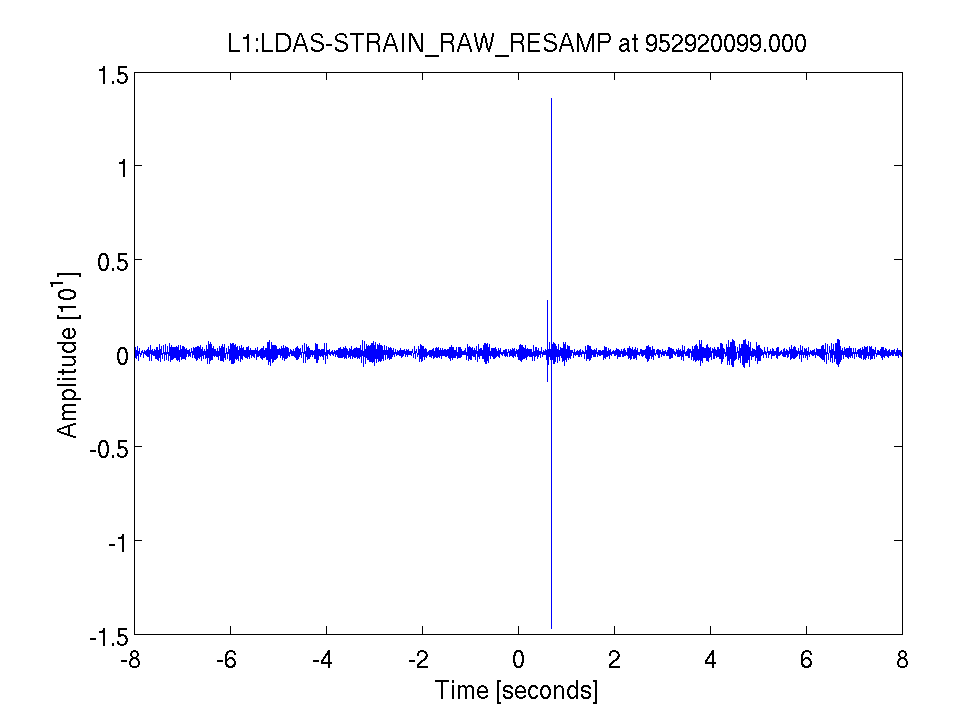
\includegraphics[width=4.75in]{figures/gating/time_series-spike.png}}
\subfigure[Gated time series.]{\label{fig:gating-time_series-gated}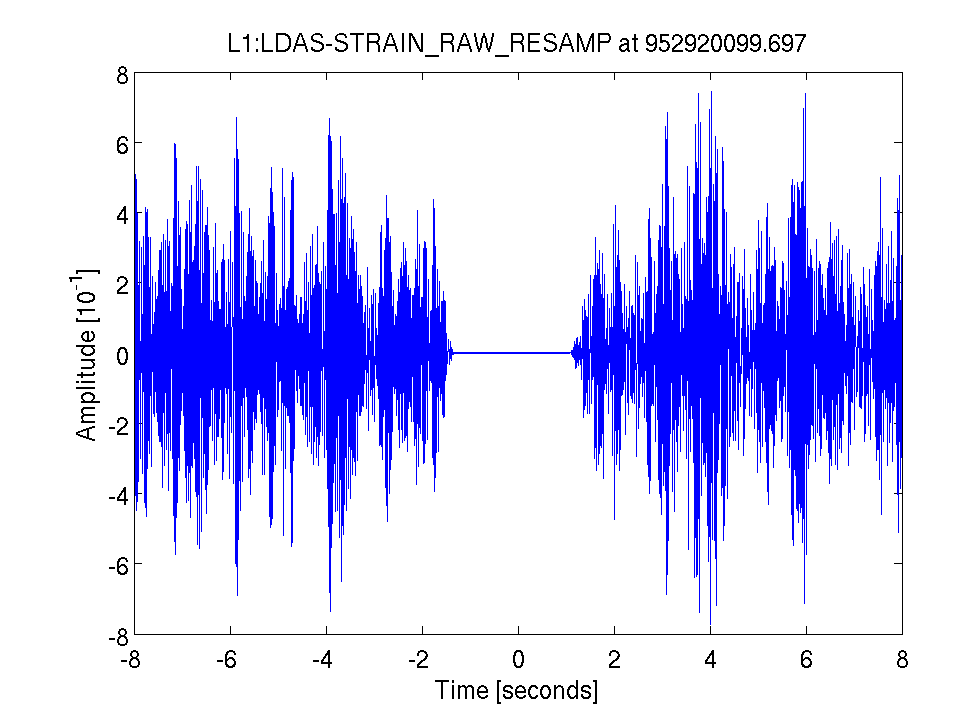
\includegraphics[width=4.75in]{figures/gating/time_series-gated.png}}
\caption{Raw and gated time series of a L1 spike glitch that occurred during
S6. In the raw time series (top) we can see that this was actually two
glitches in quick succession. For this reason, the gate was chosen to be
$\pm1.5s$ around the larger glitch. The effect of the ramping down of the Tukey
window can be seen in the gated time-series.}
\label{fig:gating-time_series}
\end{figure}

\begin{figure}[p]
\center
\subfigure[Scan with glitch in.]{\label{fig:gating-omega_scan-raw}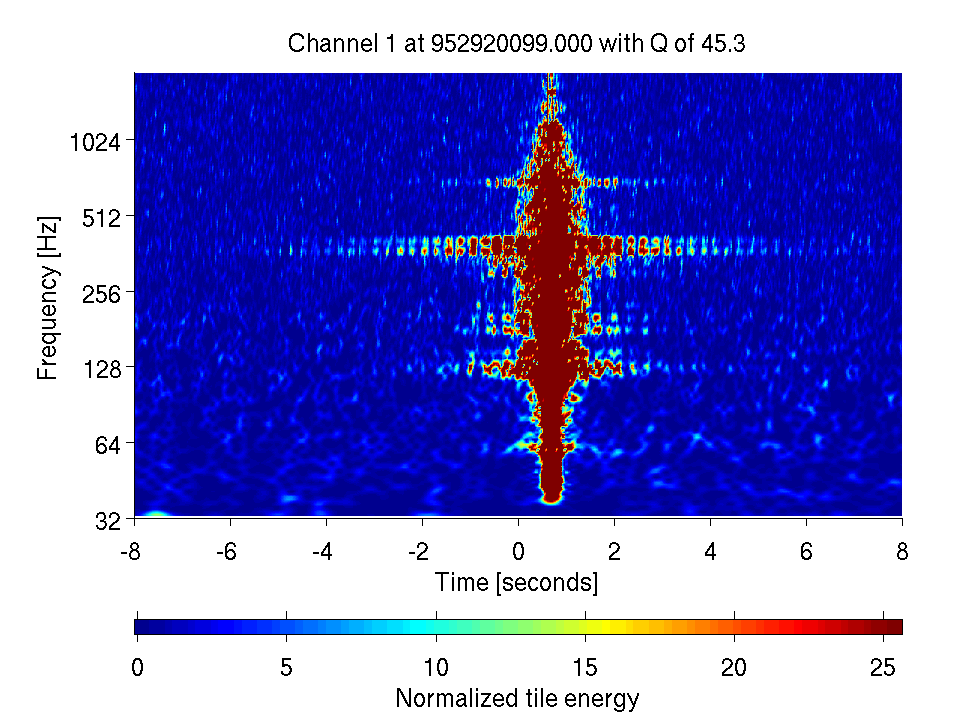
\includegraphics[width=4.75in]{figures/gating/omega_scan-spike.png}}
\subfigure[Scan with gate.]{\label{fig:gating-omega_scan-gated}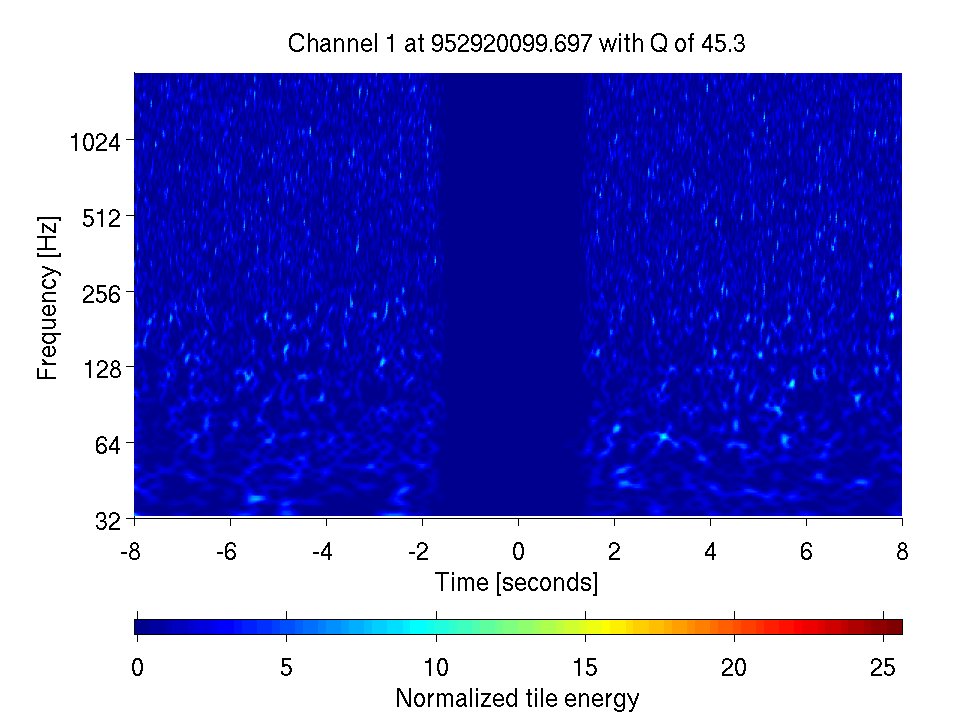
\includegraphics[width=4.75in]{figures/gating/omega_scan-gated.png}}
\caption{Omega scan of the spike glitch shown in figure
\ref{fig:gating-time_series}. The top plot shows the scan with the glitch in
the data; the bottom plot shows the scan with the glitch removed. Omega applies
a whitening filter when these scans are generated. The ``ringing" of the filter
is evident in the top plot. With the glitch gated, we see that there is no
ringing. When used in a CBC search, this implies that we would have
neither the central tower of triggers, nor the ``shoulder" and ``tail" seen in
Figure \ref{fig:spike_glitch-example}.}
\label{fig:gating-omega_scans}
\end{figure}

\section{Single Stage Pipeline and Updates to Pipedown}

Using a two stage-pipeline, as presented in chapter \ref{ch:ihope_pipeline},
makes it difficult to follow-up triggers, and to do things such as perform more
slides, as discussed in chapter \ref{ch:s6_results}. \hipe~was developed to have
two stages in order to save on the computational cost of calculating $\chi^2$.
This was done several years ago. Since then, advancements in computing speed
have made it possible to use a \emph{single-stage} pipeline. In this, $\chi^2$
is calculated at first inspiral, and so no second stage is needed. Having such
a pipeline would make it far simpler to follow-up triggers and to know how they
evolve through the pipeline.

As mentioned in \ref{ch:s6_results} a prototype single-stage pipeline already
exists. Some updates need to be made to Pipedown to be able to use this
pipeline, however, as some of the programs rely on conventions of the current
\hipe~pipeline. Of note: in the singe-stage pipeline, \verb|lalapps_thinca|
is replaced by an updated version, \verb|ligolw_thinca|, which natively makes
use of the Coinc and Experiment tables discussed in chapter
\ref{ch:ihope_pipeline}. It also performs linear slides as opposed to slides on
a ring. This removes the need for \verb|ligolw_thinca_to_coinc| in Pipedown.

A few other improvements are also planned for Pipedown. As mentioned in Chapter
\ref{ch:ihope_pipeline}, multiple veto categories can be stored in a single
database. Pipedown currently does not take advantage of this. As part of the
switch to a single-stage pipeline, we plan to add a program to Pipedown to
apply vetoes in the database, so as not to have to run \verb|ligolw_thinca|
multiple times. Also, a number of programs in Pipedown cannot read data from
multiple databases. This makes it difficult to combine results from multiple
\ihope~analysis periods. Reading from multiple databases will require a slight
update to the \verb|experiment| table. Namely, we plan to replace the
\verb|gps_start| and \verb|gps_stop| columns with a \verb|segment_def_id|
column. This would point to a list of segments in the \verb|segment| and
\verb|segment_definer| tables that give the analyzed time covered by the
database.

Pipedown can also be greatly simplified. Currently, it has to create
intermediate databases that separately store injection data from each of the
runs. These \verb|RAW| databases lack much information, such as the vetoes
applied and the live time. This is done so as to limit the size of the
\verb|LIGO_LW| XML files that need to be extracted for
\verb|lalapps_inspinjfind|. Since clustering is done on these intermediate
databases it makes it difficult to test new statistics. If one wants to cluster
with the new statistic, they must re-run clustering on all of the individual
\verb|RAW| databases, carry out injection-finding, create a new final database,
and re-compute the live time. If \verb|lalapps_inspinjfind| could read
databases instead, all of the injection runs could be added to the
\verb|FULL_DATA RAW| database at the outset, greatly simplifying the pipeline
and the ability to test new statistics. Work on this is planned. Along with
this update to the injection-finding program, we plan to implement more
sophisticated injection- finding techniques, such as using e-thinca windows.
This will decrease the chance that a glitch that occurs near the time of an
injection will be mapped to the injection, increasing confidence in ROC plots.


\section{Conclusion}

The data-analysis methods, pipeline, and search results presented in this
thesis are the result of years of work by a number of people throughout the
\ac{LSC} and the Virgo Collaboration. Although no gravitational waves have been
detected as of yet, injection studies, comparisons of our rate-upper limits to
astrophysical predictions, and the result of the \ac{S6} blind injection
challenge have made us confident that we will be able to detect when Advanced
\ac{LIGO} and Virgo come online. The work to build Advanced \ac{LIGO} is
currently underway. When it is finished it will present new challenges to our
data-analysis pipeline, some of which are outlined here. In the coming years we
will continue to improve and refine our analysis techniques to meet those
challenges, so that, when a \ac{CBC} gravitational-wave signal happens, we will
detect it.
